\section{Noise}
\label{noise}
Noise is being used to constantly send out data out to the network.
This prevents statistical analysis of the behaviour of a user and makes
de-anonmysation more unpractical due to the amount of data that needs
to be tracked and analysed.
%There are many situations in which an EOFi sends out data to the network,
%although you did not write a message: In fact, as EOFi \textbf{always}
%sends packets in a fixed interval, it needs to have data to encrypt and send.
Furthermore noise is used to fill in the unused fields in the EOF messages.
Noise can be any type of random data. As the current random number generators
are quite expensive, it is recommend to use a huge dictionary, old 
messages, logfiles, public emails, etc. for noise input.
The reference implementation uses the archive of RFCs as base for noise.
The noise workflow is shown in figure \ref{noiseworkflow}.
\begin{figure}
    \centering
    \caption{Noise Workflow}
    \label{noiseworkflow}
    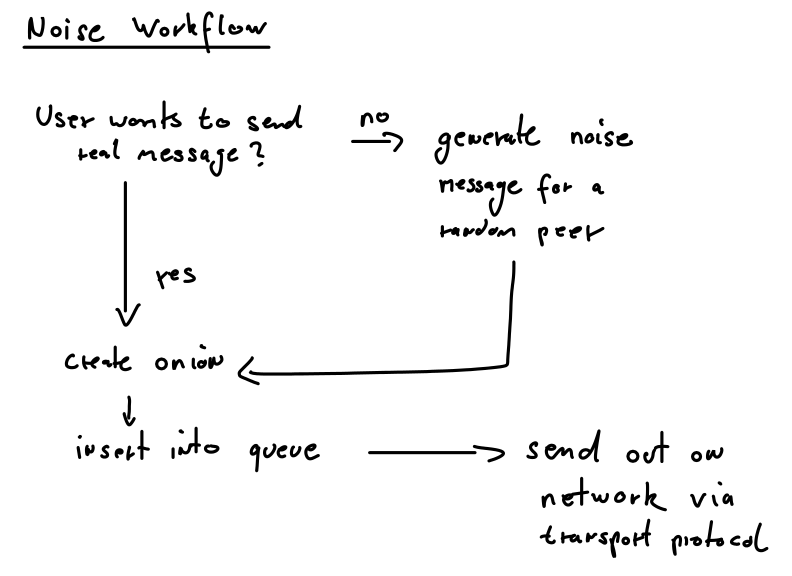
\includegraphics[scale=0.8]{noiseworkflow.png}
\end{figure}

% ----------------------------------------------------------------------------
\subsection{Latency}
\label{latency}
Latency is important for the user experience of the chat system.
This is especially important after the initial \textit{human handshake}
of saying hello has been made (before nobody knows when to expect
a message).
\textit{System Response Time and User Satisfaction}\cite{responsetime}
indicates that response times up to 6 seconds are tolerable. These numbers
cannot be related directly to the tolerated delay, because the receiving
peer does not exactly know when the she can expect the sending peer to write
a message.
Every additional proxy peers adds an amount of time to the latency until the
message arrives, as can be seen below.
% ----------------------------------------------------------------------------
\subsubsection{Average Latency}
The average latency for a peer is calculated as follows (+1 is needed to
included the receiving peer itself):
$$\frac{\sum\limits_{i=0}^{(Proxy peers count +1)}}{Proxy peers count + 1}$$
Depending on the sending interval this results in different average
waiting times for message to arrive, as expressed in
the following formula:
$$Intervaltime * \frac{\sum\limits_{i=0}^{(Proxy peers +1)}}{Proxy peers + 1}$$
The average latency depending on the number of hosts and the sending interval
used is shown in table \ref{avglatencypeers}.
\begin{longtable}{|c|c|c|c|c|c|c|}
\caption{Average latency based on number of proxy peers}
\label{avglatencypeers}\\
\hline
\multirow{2}{*}{\textbf{Proxy peers}} & \multicolumn{6}{|l|}{\textbf{Average latency (multiplied by delay times)}} \\
& \textbf{(\# timeslots)} & \textbf{0.125s} & \textbf{0.25s} & \textbf{0.5s} & \textbf{1s} & \textbf{2s}\\
\hline
\textbf{1} & 0.5 & 0.0625s & 0.125s & 0.25s & 0.5s & 1s\\
\hline
\textbf{2} & 1 & 0.125s & 0.25s & 0.5s & 1s & 2s\\
\hline
\textbf{3} & 1.5 & 0.1875s & 0.375s & 0.75s & 1.5s & 3s\\
\hline
\textbf{4} & 2 & 0.25s & 0.5s & 1s & 2s & 4s\\
\hline
\textbf{5} & 2.5 & 0.3125s & 0.625s & 1.25s & 2.5s & 5s\\
\hline
\textbf{6} & 3 & 0.375s & 0.75s & 1.5s & 3s & 6s\\
\hline
\textbf{7} & 3.5 & 0.4375s & 0.875s & 1.75s & 3.5s & 7s\\
\hline
\textbf{8} & 4 & 0.5s & 1s & 2s & 4s & 8s\\
\hline
\textbf{9} & 4.5 & 0.5625s & 1.125s & 2.25s & 4.5s & 9s\\
\hline
\textbf{10} & 5 & 0.625s & 1.25s & 2.5s & 5s & 10s\\
\hline
\end{longtable}
% ----------------------------------------------------------------------------
\subsubsection{Maximum Latency}
Furthermore besides the average latency, the maximum latency needs
to be taken into account as well, which is shown in table \ref{maxlatencypeers}.
\begin{longtable}{|c|c|c|c|c|c|c|}
\caption{Maximum latency based on number of proxy peers}
\label{maxlatencypeers}\\
\hline
\multirow{2}{*}{\textbf{Proxy peers}} & \multicolumn{6}{|l|}{\textbf{Maximum latency (multiplied by delay times)}} \\
& \textbf{(\# timeslots)} & \textbf{0.125s} & \textbf{0.25s} & \textbf{0.5s} & \textbf{1s} & \textbf{2s}\\
\hline
\textbf{1} & 1 & 0.125s & 0.25s & 0.5s & 1s & 2s\\
\hline
\textbf{2} & 2 & 0.25s & 0.5s & 1s & 2s & 4s\\
\hline
\textbf{3} & 3 & 0.375s & 0.75s & 1.5s & 3s & 6s\\
\hline
\textbf{4} & 4 & 0.5s & 1s & 2s & 4s & 8s\\
\hline
\textbf{5} & 5 & 0.625s & 1.25s & 2.5s & 5s & 10s\\
\hline
\textbf{6} & 6 & 0.75s & 1.5s & 3s & 6s & 12s\\
\hline
\textbf{7} & 7 & 0.875s & 1.75s & 3.5s & 7s & 14s\\
\hline
\textbf{8} & 8 & 1s & 2s & 4s & 8s & 16s\\
\hline
\textbf{9} & 9 & 1.125s & 2.25s & 4.5s & 9s & 18s\\
\hline
\textbf{10} & 10 & 1.25s & 2.5s & 5s & 10s & 20s\\
\hline
\end{longtable}
% ----------------------------------------------------------------------------
\subsection{Bandwidth Usage}
\label{bwusagetheory}
Based on the calculated packet sizes (section \ref{pkgsizes}, p. \pageref{pkgsizes}), 
the following \textbf{outgoing bandwidth}
is needed, as can be seen in table \ref{bandwidth}.
The highest needed bandwidth
in case of 10 proxy peers sending at an interval of 0.125s results in 64 KiB/s
(aequivalent of 512 KBit/s).
 Todays DSL connections usually exceed this limit by magnitudes.
\begin{longtable}{|c|c|c|c|c|c|}
\caption{Outgoing bandwidth usage}
\label{bandwidth}\\
\hline
\multirow{2}{*}{\textbf{Proxy peers}} & \multicolumn{5}{|l|}{\textbf{Intervals / Bandwidth usage in KiB/s}} \\
& \textbf{0.125s} & \textbf{0.25s} & \textbf{0.5s} & \textbf{1s} & \textbf{2s}\\
\hline
\textbf{1} & 9.6 & 4.8 & 2.4 & 1.2 & 0.6\\
\hline
\textbf{2} & 15.2 & 7.6 & 3.8 & 1.9 & 0.95\\
\hline
\textbf{3} & 20.8 & 10.4 & 5.2 & 2.6 & 1.3\\
\hline
\textbf{4} & 26.4 & 13.2 & 6.6 & 3.3 & 1.65\\
\hline
\textbf{5} & 32 & 16 & 8 & 4 & 2\\
\hline
\textbf{6} & 38.4 & 19.2 & 9.6 & 4.8 & 2.4\\
\hline
\textbf{7} & 44.8 & 22.4 & 11.2 & 5.6 & 2.8\\
\hline
\textbf{8} & 50.4 & 25.2 & 12.6 & 6.3 & 3.15\\
\hline
\textbf{9} & 56.8 & 28.4 & 14.2 & 7.1 & 3.55\\
\hline
\textbf{10} & 64 & 32 & 16 & 8 & 4\\
\hline
\end{longtable}
Even on mobile networks, HSUPA Category 1 delivers 0.73 Mbit/s upstream bandwidth.
Older ISDN and Modem connections would not suffice, though
today there are a lot of alternative connections
 available.\cite{wiki:bitrates}
If using only 9 proxy servers with 0.125s delay or
10 proxy servers with a delay of 0.25s, EDGE could be supported.

The total required network bandwidth is the product of peers in the
network multiplied by the outgoing bandwidth per peer:
$$Required Network Bandwidth = Network Peers * Peer Bandwidth$$
Thus a network with 100 peers, all of them which use 10 proxy peers
and send at a rate of 0.125s, the total required network bandwidth would be
$$RNB = 100 * 64 KiB/s = 6400 KiB/s = 6.25MiB/s = 50 MBit/s$$
If also the receiving side is inside the same network, the required network
bandwith has to be multiplied by two and thus results in 
\textit{100 MBit/s}. This is exactly half of what a fast ethernet switch
can deliver, because fast ethernet provides full duplex 100Mbit/s streams
and thus a single fast ethernet fabric would support 200 simultaneous users.
As the network bandwidth cannot be controlled or influenced by the user
directly, these calculations may simply indicate the network bandwidth
usage for network providers. The user can focus on the bandwith specifications
found in table \ref{bandwidth}.
% ----------------------------------------------------------------------------
\subsection{Fixed interval for sending}
To prevent de-anonymisation by doing statistical analysis on the traffic,
postcards are being send at a fixed rate.
In case there is not message to be send, onions with no receiving
peer (\textit{noise}) must be used instead.

To avoid problems with different sending intervals
(queuing, buffer exceeding) a network wide fixed sending interval
should be chosen. From the calculations made above, an interval
of \textbf{0.25s} seems to provide a good tradeoff between
latency, anonymity and bandwidth usage.

The number of proxy peers can be choosen by every peer individually
and can be used to focus on smaller bandwidth usage and less latency
or a higher degree of anonymity. A value of 5 in a network of 100 peers
would make de-anonymising less probable than winning Lotto in Germany
(6 of 49).
